%======================================================================
% L10_SF_canon_ensemble.pdf
%======================================================================
% škrtnutí (krácení) v rovnicích -- bez balíčku cancel
\providecommand{\cancel}[1]{\tikz[baseline=(c.base)]{\node[inner sep=0pt] (c) {$\displaystyle #1$}; \draw (c.south west) -- (c.north east);}}
\section{Mikrokanonický a kanonický soubor}

%----------------------------------------------------------------------
\strana{L10-1}
\subsection*{Mikrokanonický soubor}
\begin{itemize}
  \item popisuje \kw{izolovaný systém} ($E, V, N$ konstantní)
  \item hustota pravděpodobnosti mikrostavů na fáz.\ prostoru je konstantní:
\end{itemize}

\begin{minipage}{0.68\textwidth}
\[
  \vzorec{\textcolor{OliveGreen}{w(\mathbf p,\mathbf q; E,V,N) = \frac{1}{\Sigma(E,V,N)}\,\delta\big[E - H(\mathbf p,\mathbf q)\big]}}
\]
\begin{center}(\kw{princip stejných pravděpodobností})\end{center}
\end{minipage}
\begin{minipage}{0.3\textwidth}
\textcolor{NavyBlue}{\textcircled{\small$*$} \underline{Boltzmann:} \\
Permutabilitätmass \\
\hspace*{1.2cm}$\shortparallel$ \\
permutability measure}
\end{minipage}

\begin{itemize}
  \item $\Sigma(E,V,N) = \int\dd\tau_N\,\delta\big[E - H(p,q)\big]$ je v nějakém smyslu mírou pravděpodobnosti\textsuperscript{\textcolor{NavyBlue}{($*$)}} makrostavu \dots\ pokud by systém procházel celý fázový prostor zcela náhodně bez omezení na $E$, potom $\Sigma(E,V,N)/\Sigma_{tot}$ je pst., že ho najdeme právě v $M = (E,V,N)$
        \textcolor{NavyBlue}{-- dává samozřejmě lepší smysl, pokud vztáhneme k jinému TD param.\ než $E$ \dots}
  \item o jak velkých číslech se bavíme: $N\sim N_A = 10^{23}$, každá částice se může nacházet pouze ve 2 stavech $\Rightarrow$ \textcolor{Red}{$\Omega\sim 2^{10^{23}}$!}
  \item \underline{entropie mikrokanon.\ souboru} je
  \[
    \vzorec{S(E,V,N) = k_B\log\Sigma(E,V,N)} \qquad (*)
  \]
  \[
    \Updownarrow
  \]
  \[
    \Sigma(E,V,N) = \exp\Big(\frac{1}{k_B}S(E,V,N)\Big)
  \]
  \item $(*)$ je entropická fundamentální rovnice \\
        $\to$ lze plně aplikovat formalismus TD
        \[
          \to\quad \frac1T \equiv \pdv{S}{E} \qquad \frac{p}{T} = \pdv{S}{V} \qquad -\frac{\mu}{T} = \pdv{S}{N}
        \]
        $\to$ rovnováha definována rovností intenzivních parametrů
\end{itemize}

\textcolor{NavyBlue}{\underline{NB:} lze psát \ $S(E) = k_B\log\Sigma(E) = -k_B\displaystyle\int_{H=E}\dd\tau_N\,w(p,q)\log w(p,q)$}

%----------------------------------------------------------------------
\strana{L10-2}
\begin{itemize}
  \item \underline{mikrokanonický soubor a interagující systémy} \\
        z druhé strany:
  \begin{itemize}[label=$\to$]
    \item uvažujme 2 izolované systémy s energiemi $E_1$ a $E_2$
    \item $(1)\leftrightarrow\Sigma_1(E_1)$ \ \& \ $S_1(E_1) = k_B\log\Sigma_1(E_1)$ \\
          $(2)\leftrightarrow\Sigma_2(E_2)$ \ \& \ $S_2(E_2) = k_B\log\Sigma_2(E_2)$
    \item systémy neinteragují, jsou nezávislé $\Rightarrow$ pro složený systém platí ($E_{tot} = E_1 + E_2$)
          \[
            \Sigma(E_1,E_2) = \Sigma_1(E_1)\Sigma_2(E_2) \ \Rightarrow\ S(E_1,E_2) = S_1(E_1) + S_2(E_2)
          \]
          \pozn{v originále $S_2(E_1)$ -- zjevný překlep}
    \item systémy uvedeme do kontaktu tak, že si mohou vyměňovat energii \\
          $\Rightarrow$ $E_{tot} = E_1 + E_2$ se zachová, ale objem fáz.\ prostoru pro kompozitní systém se enormně zvětší:
          \hfill (zde předpokládám slabou interakci)
  \end{itemize}
\end{itemize}

\begin{minipage}{0.68\textwidth}
\[
  \Sigma(E_{tot}) = \int_0^{E_{tot}}\dd E_1'\,\Sigma_1(E_1')\,\Sigma_2(E_{tot} - E_1')
\]
\end{minipage}
\begin{minipage}{0.3\textwidth}
$H = H_1 + H_2 + V$ \\
\& $E\sim\langle H_1\rangle + \langle H_2\rangle$ \\
\hspace*{0.9cm}$E_1 \quad + \quad E_2$
\end{minipage}
\[
  = \Big/\ \Sigma_i(E_i) = \exp\Big(\frac{1}{k_B}S_i(E_i)\Big)\ \Big/ \ \Rightarrow
\]
\[
  \Sigma(E_{tot}) = \int\dd E_1'\,\exp\Big(\frac{1}{k_B}S_1(E_1') + \frac{1}{k_B}S_2(E_{tot} - E_1')\Big) \qquad (*)
\]

\begin{itemize}[label=$\to$]
  \item zjevně platí
  \[
    S_{tot}(E_{tot}) = k_B\log\Sigma(E_{tot}) \geq \underbrace{S_1(E_1) + S_2(E_2)}_{\text{původní stav}}
  \]
  \item $S_i\propto N_i\sim N_A$ $\Rightarrow$ integrál $(*)$ je zcela dominován maximem argumentu v exp: \ $(S_1 + S_2)^{max} = \epsilon(S_1 + S_2)$ \\
        $\Rightarrow$ \quad $\exp(S_1 + S_2)^{max} = e^{\epsilon N_A}\exp(S_1 + S_2)$ \\
        (viz metoda sedlového bodu)
\end{itemize}

%----------------------------------------------------------------------
\strana{L10-3}
{\color{NavyBlue}
\[
  \Sigma(E_{tot}) = \int\dd E_1'\,\exp\Big(\frac{1}{k_B}S_1(E_1') + \frac{1}{k_B}S_2(E_{tot} - E_1')\Big) \equiv I
\]
\[
  g(E') = \frac{1}{k_B}\big[S_1(E') + S_2(E_{tot} - E')\big]
  \qquad\Rightarrow\quad E^*:\ \ \pdv{S_1(E)}{E}\Big|_{E=E^*} = \pdv{S_2(E)}{E}\Big|_{E=E^*}
\]
\[
  \Rightarrow\quad g(E') = g(E^*) - \tfrac12|g''(E^*)|(E - E^*)^2
\]
\[
  g'' = \pdv{E}\Big(\frac{1}{T_1(E)} - \frac{1}{T_2(E_{tot} - E)}\Big)
\]
\[
  \Rightarrow\quad I = \exp\Big[\frac{1}{k_B}\big(S_1(E^*) + S_2(E_{tot} - E^*)\big)\Big]\cdot
  \underbrace{\int_0^\infty\dd E'\exp\Big(-\frac{|g''(E^*)|}{2k_B}(E - E^*)\Big)}_{\leq\sqrt{\frac{2\pi k_B}{|g''(E^*)|}}}
\]
\[
  g''\propto N^{-1}
\]
\[
  \Rightarrow\quad I\propto\exp(N)\times N^{1/2}
  \quad\Rightarrow\quad S_{tot}\sim\log I \propto \underset{\substack{\uparrow\\ \text{příspěvek čistě od } E^*!}}{N} + \tfrac12\log N
\]
}
\pozn{v exponentu integrálu v originále $(E-E^*)$ bez kvadrátu -- ponecháno}

%----------------------------------------------------------------------
\strana{L10-4}
\begin{veta}[Rovnováha dvou systémů -- maximum entropie]
\begin{itemize}
  \item def.\ $E_*$: \quad $\displaystyle\pdv{S_1}{E_1}\Big|_{E_*} - \pdv{S_2}{E_2}\Big|_{E_{tot} - E_*} = 0$
\end{itemize}
\[
  \Rightarrow\quad \vzorec{S(E_{tot}) \simeq S_1(E_*) + S_2(E_{tot} - E_*) \geq S_1(E_1) + S_2(E_2)}
\]
\end{veta}

\textcolor{Red}{\small Zde je zajímavý detail: $E^*$ interpretujeme jako makroskop.\ pozorovanou $E_1$, to by ale měla být střední hodnota $\langle E_1\rangle$; my ji zde aproximujeme modem (nejpravděpodobnější hodnotou), což je nicméně až na příspěvky úměrné $\log(N)$ v pořádku, viz obrázek níže a centrální limitní věta}

\begin{itemize}
  \item dostáváme \kw{2.\ TDZ}
  \item argumentace znovu ukazuje jeho statistickou interpretaci: systém (1) se může nacházet s nějakou pravděpodobností v libovolném $M$-stavu, s naprosto dominantní pravděpodobností se však bude nacházet ve stavu $E_1 = E_*$
\end{itemize}

\begin{minipage}{0.55\textwidth}
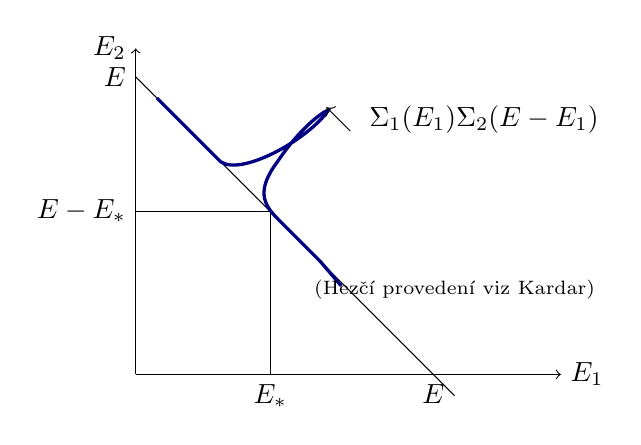
\begin{tikzpicture}[scale=0.9]
  \draw[->] (0,0) -- (6,0) node[right] {$E_1$};
  \draw[->] (0,0) -- (0,4.6) node[left] {$E_2$};
  \draw (0,4.2) -- (4.5,-0.3);
  \node[left] at (0,4.2) {$E$};
  \node[below] at (4.2,0) {$E$};
  % E_* projekce
  \draw (1.9,0) -- (1.9,2.3) -- (0,2.3);
  \node[below] at (1.9,0) {$E_*$};
  \node[left] at (0,2.3) {$E - E_*$};
  % Sigma1 Sigma2 - ostrý pík kolmo k přímce
  \draw[NavyBlue,very thick] (0.3,3.9) -- (1.2,3.0)
     .. controls (1.5,2.8) and (2.4,3.3) .. (2.7,3.7)
     .. controls (2.8,3.8) and (2.4,3.6) .. (2.0,3.0)
     .. controls (1.7,2.6) and (1.8,2.4) .. (2.0,2.2)
     -- (2.6,1.6) -- (2.9,1.25);
  \node at (4.6,3.6) {$\nwarrow\ \Sigma_1(E_1)\Sigma_2(E - E_1)$};
  \node at (4.5,1.2) {\scriptsize (Hezčí provedení viz Kardar)};
\end{tikzpicture}
\end{minipage}
\begin{minipage}{0.43\textwidth}
\small It's worth stressing that there is no a priori reason why the first system should have a fixed energy once it is in contact with the second system. But the large number of particles involved means that it is overwhelmingly likely to be found with energy $E_\star$ which maximises the number of states of the combined system. Conversely, once in this bigger set of states, it is highly unlikely that the system will ever be found back in a state with energy $E_1$ or, indeed, any other energy different from $E_\star$.

It is this simple statement that is responsible for all the irreversibility that we see in the world around us. This is the \emph{second law of thermodynamics}. As a slogan, ``entropy increases''. When two systems are brought together --- or, equivalently, when constraints on a system are removed --- the total number of available states available is vastly enlarged.
\end{minipage}

\subsection*{\textcolor{NavyBlue}{Sumace/integrace exponenciál:}}
{\color{NavyBlue}
\textbf{1)} \quad $\Gamma = \displaystyle\sum_{i=1}^{M}\Omega_i$ \qquad $\Omega_i\sim\exp(N\phi_i)$ \qquad $M\sim N^\alpha$ \qquad $N\gg 1$ \ ($N\sim N_A$)
\begin{itemize}
  \item $0\leq\Omega_i\leq\Omega_{max}$ \quad $\Rightarrow$ \quad $\Omega_{max}\leq\Gamma\leq M\,\Omega_{max}$
  \item uvažujme $\frac1N\log\Gamma$:
\end{itemize}
}

\begin{center}
\begin{minipage}{0.9\textwidth}
\small The phrase ``highly unlikely'' is used only because the English language does not contain enough superlatives to stress how ridiculously improbable a violation of the second law would be. The silly number of possible states in a macroscopic systems means that violations happen only on silly time scales: exponentials of exponentials. This is a good operational definition of the word ``never''.
\end{minipage}
\end{center}

{\color{NavyBlue}
\[
  \frac1N\log\Omega_{max} \leq \frac1N\log\Gamma \leq \frac1N\log M\Omega_{max} = \frac1N\log\Omega_{max} + \frac{\alpha}{N}\log N
\]
\[
  \Big\downarrow\ N\to\infty
\]
\[
  \lim_{N\to\infty}\frac1N\log\Omega_{max} \leq \frac1N\log\Gamma \leq \frac1N\log\Omega_{max}
\]
\[
  \Rightarrow\quad \vzorec{\lim_{N\to\infty}\frac1N\log\Gamma = \lim_{N\to\infty}\frac1N\log\Omega_{max} = \phi_{max}}
\]

\textbf{2)} \quad $I = \displaystyle\int\dd x\,\exp\big(N\phi(x)\big) = \int\dd x\,\exp\Big(N\phi(x_{max}) - \frac{N}{2}\phi''(x_{max})(x - x_{max})^2 + \dots\Big)$
\[
  \Rightarrow\quad I\sim\exp\big(N\phi(x_{max})\big)
  \underbrace{\int\dd x\,\exp\Big(-\frac{N}{2}\phi''(x_{max})(x - x_{max})^2\Big)}_{\sqrt{\frac{2\pi}{N\phi''}}}
  \propto\frac{1}{\sqrt N}\exp\big(N\phi(x_{max})\big)
\]
\[
  \Rightarrow\quad \lim_{N\to\infty}\frac{\log I}{N} = \lim_{N\to\infty}\Big(\phi(x_{max}) - \frac12\frac{\log N}{N}\Big) = \phi(x_{max})
\]
}

%----------------------------------------------------------------------
\strana{L10-5}
\subsection{Kanonický soubor}
\begin{itemize}
  \item popis systému v kontaktu s \kw{tepelnou lázní}
  \item uvažujme \underline{izolovaný kompozitní systém složený z podsystému a mnohem většího rezervoáru}:
  \begin{itemize}[label=$\to$]
    \item $E_T = E + E_R = \text{konst}$ \qquad $E\ll E_R$, \quad $N\ll N_R$
    \item $S_R = k_B\log\Sigma_R(E_R) \gg S = k_B\log\Sigma(E,V,N)$
  \end{itemize}
  \item pravděpodobnost realizace konkrétní distribuce energie $E_T = E + E_R$ je \ $P(E|E_T) = w(E|E_T)\,\dd E$
\end{itemize}
\[
  w(E,V,N|E_T) = \frac{\Sigma(E,V,N)\,\Sigma_R(E_T - E)}{\Sigma_T(E_T)}
\]
\hspace*{2.2cm}\textcolor{NavyBlue}{$\nwarrow$ hustota podmíněné pravděpodobnosti}
\begin{align*}
  \Rightarrow\quad S_{tot}(E_T) &= k_B\log\Sigma_T(E_T) \\
  &= k_B\log\Sigma(E) + k_B\log\Sigma_R(E_T - E) - k_B\log w(E;E_T) \\
  &> S(E) + S_R(E_T - E)
\end{align*}
\[
  \Rightarrow\quad \log w(E|E_T) = \log\Sigma(E) + \log\Sigma_R(E_T - E) - \log\Sigma_T(E_T)
\]
{\color{NavyBlue}
\[
  \Big/\ E_T\gg E \ \Rightarrow\ \log\Sigma_R(E_T - E) = \log\Sigma_R(E_T) - E\,\pdv{\log\Sigma_R(E_R)}{E_R}\Big|_{E_R = E_T}
\]
\[
  \pdv{\log\Sigma_R(E_R)}{E_R} = \frac{1}{k_B}\pdv{S_R(E_R)}{E_R} = \frac{1}{k_BT_R} \equiv \beta_R
  \qquad \begin{pmatrix} E_T\to E_T - E \\ \Downarrow \\ \beta_R\simeq\beta_R\end{pmatrix}
\]
\begin{itemize}
  \item jakou chybu dělám? \\
        oprava je \ $E^2\,\dfrac{\partial^2\log\Sigma_R(E_R)}{\partial E_R^2} = \mathcal{O}\Big(\epsilon\,\dfrac{E}{E_T}\Big)$, tedy \\
        $\Big(\epsilon = \dfrac{E}{E_T}\Big)\times$ menší než vedoucí $\dfrac{E}{k_BT}$
\end{itemize}
}

%----------------------------------------------------------------------
\strana{L10-6}
\[
  \Rightarrow\quad \log w(E|E_T) = \log\Sigma(E) - \beta_RE - \log\frac{\Sigma_T(E_T)}{\Sigma_R(E_T)}
\]
{\color{OliveGreen}
\textbf{Def:} \quad $\beta \equiv \dfrac{1}{k_BT}$
\[
  \log Z_c(E_T) = \log\frac{\Sigma_T(E_T)}{\Sigma_R(E_T)} \quad\dots\ \text{z hlediska podsystému je to konstanta}
\]
}
\begin{veta}[Kanonické rozdělení]
\[
  \Rightarrow\quad \vzorec{\textcolor{OliveGreen}{w_c(E|E_T) = \frac{1}{Z_c(E_T)}\,\Sigma(E)\,e^{-\beta E}}}
  \qquad \text{v rovnováze } T = T_R \ \Rightarrow\ \beta_R = \beta
\]
\end{veta}

\begin{itemize}
  \item $Z$ zde hraje roli normalizační konstanty a tedy lze vyjádřit jako $\big(\int w(E)\,\dd E = 1\big)$
\end{itemize}

\begin{minipage}{0.68\textwidth}
\[
  \vzorec{Z_c(\beta,V,N) = \int_0^{\textcolor{NavyBlue}{E_T\to\infty}}\dd E\,\Sigma(E,V,N)\,e^{-\beta E}}
\]
\end{minipage}
\begin{minipage}{0.3\textwidth}
\small\textcolor{NavyBlue}{$E_T$ již explicitně nevystupuje, je nahrazena teplotou $\Rightarrow$} \\
\textcolor{OliveGreen}{$w_c(E|E_T) = w(E|\beta)$}
\end{minipage}

\underline{NB:}
\begin{itemize}[nosep]
  \item $Z(\beta,V,N)$ je \kw{Laplaceova transformace} $\Sigma(E,V,N)$
  \item \underline{Zustandsumme} -- \kw{partiční suma/funkce}
  \begin{itemize}[nosep]
    \item[--] uvidíme, že obsahuje veškerou relevantní fyzikální informaci $\Rightarrow$ centrální objekt SF
  \end{itemize}
  \item jak je to s horní mezí $E_T\to+\infty$:
  \begin{itemize}[nosep,label=$\to$]
    \item striktně vzato může být $E\leq E_T < +\infty$
    \item je-li $H$ shora neomezený, potom $\Sigma(E)$ je monot.\ rostoucí funkce $E$
    \item \underline{id.\ plyn}: \quad $\Sigma\propto E^{\frac32N} = E^{N\frac f2}$ \qquad $f$ \dots\ počet st.\ volnosti
    \item obecně lze předpokládat $\Sigma\propto E^{qN}$
          \[
            \Rightarrow\quad E^{qN}e^{-\beta E} \xrightarrow{\ E\nearrow\ } e^{-\beta E} \xrightarrow{\ E\to E_T\ } 0
          \]
          \[
            \Rightarrow\quad \int^{E_T} = \int^{+\infty}
          \]
  \end{itemize}
\end{itemize}

%----------------------------------------------------------------------
\strana{L10-7}
\quad $\to$ fyzikálně: je-li $R\gg S$, potom je jistě efektivně nulová pst $E_R = 0$ \& $E = E_T$

\begin{center}
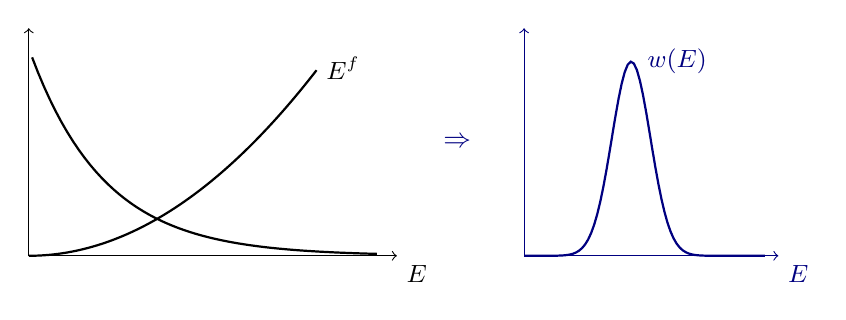
\begin{tikzpicture}[scale=0.85]
  % levý graf
  \draw[->] (0,0) -- (5.5,0) node[below right] {\small $E$};
  \draw[->] (0,0) -- (0,3.4);
  \draw[thick,domain=0.05:5.2,samples=60] plot (\x,{3.1*exp(-0.9*\x)});
  \draw[thick,domain=0:4.3,samples=60] plot (\x,{0.15*\x*\x});
  \node[right] at (4.3,2.8) {\small $E^f$};
  \node at (6.4,1.7) {\textcolor{NavyBlue}{$\Rightarrow$}};
  % pravý graf
  \begin{scope}[xshift=7.4cm,NavyBlue]
    \draw[->] (0,0) -- (3.8,0) node[below right] {\small $E$};
    \draw[->] (0,0) -- (0,3.4);
    \draw[thick,domain=0:3.6,samples=80] plot (\x,{2.9*exp(-6*(\x-1.6)*(\x-1.6))});
    \node[right] at (1.7,2.9) {\small $w(E)$};
  \end{scope}
\end{tikzpicture}
\end{center}

\begin{itemize}
  \item je zřejmé, že $\Sigma(E,V,N)\to Z_c(\beta,V,N)$ úzce souvisí s \kw{Legendreovou transformací} $U\leftrightarrow T$ resp.\ $S\leftrightarrow\frac1T$ v termodynamice -- zde pracujeme se stejným podsystémem, jaký v TD popisujeme fund.\ rovnicí $F(T,V,N)$ resp.\ $S[\frac1T](\frac1T,V,N)$
  \item $w(E)$ definuje \underline{kanonický} statistický \underline{soubor}
  \begin{itemize}[label=$\to$]
    \item opět uvažujeme veliké množství kopií sledovaného makroskopického systému, ovšem hustota pstí není uniformní -- závisí na energii tak, že systém má definovanou teplotu $k_BT = \frac1\beta$
    \item energii může vyměňovat s rezervoárem $\Rightarrow$ tato je určena pouze střední hodnotou
    \[
      \vzorec{\langle E\rangle = \int\dd\tau_N\,w_c(p,q)\,H(p,q) = \int\dd E\,w_c(E;\beta)\,E}
    \]
    \hspace*{3.8cm}$\uparrow$ kanonická hustota pravděpodobnosti na fáz.\ prostoru
    \item $w_c(p,q;\beta,X_1,\dots,X_a)$ závisí parametricky na teplotě \& extenzivních parametrech určujících rovnovážný makrostav (pod)systému
    \item jako ve $F(T,V,N)$, role rezervoáru se redukuje na fixaci teploty
  \end{itemize}
\end{itemize}

%----------------------------------------------------------------------
\strana{L10-8}
\subsubsection*{Kanonická hustota psti ve fáz.\ prostoru}
\begin{itemize}
  \item hustota psti pro celý složený systém:
  \[
    w_\mu(p,q;p_R,q_R) = \frac{1}{\Sigma_T(E_T)}\,\delta\big(E_T - H(p,q) - H_R(p_R,q_R)\big)
  \]
  \item integrál přes mikrostavy rezervoáru:
  \[
    w_c(p,q) = \int\dd\tau_{N_R}\,w_\mu(p,q;p_R,q_R) = \frac{\Sigma_R\big(E_T - H(p,q)\big)}{\Sigma_T(E_T)}
  \]
  \hspace*{2.6cm}\textcolor{NavyBlue}{$\uparrow$ může být $\frac{1}{N_R!}$ (je-li rez.\ plyn nerozliš.\ částic)}
  \item v relevantní oblasti fáz.\ prostoru je $H(p,q)\ll E_T$ $\to$
\end{itemize}
\[
  \log w_c(p,q) \doteq \log\Sigma_R(E_T) - H(p,q)\,\pdv{\log\Sigma_R(E_R)}{E_R}\Big|_{E_T} - \log\Sigma_T(E_T)
\]
\[
  \log w_c(p,q) = -\beta_RH(p,q) - \log\frac{\Sigma_T(E_T)}{\Sigma_R(E_T)} \equiv -\beta H(p,q) - \log Z_c
\]
\begin{veta}[Kanonická hustota pravděpodobnosti]
\[
  \Rightarrow\quad \vzorec{w_c(p,q;\beta) = \frac{1}{Z_c(\beta,V,N)}\,e^{-\beta H(p,q)}};
  \qquad \vzorec{Z_c(\beta,V,N) = \textcolor{Red}{\cancel{\tfrac{1}{N!}}}\int\dd\tau_N\,e^{-\beta H(p,q)}}
\]
\textcolor{Red}{\small$\uparrow$ obsaženo v $\dd\tau_N$?}
\end{veta}
\textcolor{NavyBlue}{NB: kompatibilní s \ $\langle E\rangle = \int\dd\tau_N\,w_c(p,q)\,H(p,q) = \int\dd E\,w_c(E)\,E$}

\subsection{Kanonický soubor \& termodynamika}
\begin{minipage}{0.6\textwidth}
\begin{itemize}
  \item \underline{fundamentální rovnice}
\end{itemize}
\end{minipage}
\begin{minipage}{0.38\textwidth}
\textcolor{Red}{\underline{Pozn:} $\frac{1}{N!}\dd\tau_N\to\dd\tau_N$ \\ (kombinatorický faktor zahrnuji do $\dd\tau_N$)}
\end{minipage}

\begin{minipage}{0.6\textwidth}
\begin{align*}
  Z_c &= \int\dd E\,\Sigma(E,V,N)\,e^{-\beta E} \\
  w(E,V,N) &= \frac{1}{Z_c}\,\Sigma(E,V,N)\,e^{-\beta E}
\end{align*}
\end{minipage}
\begin{minipage}{0.38\textwidth}
\begin{tcolorbox}[colback=white,colframe=black,boxrule=0.5pt,sharp corners]
\centering mikrokan.\ soubor \\ $\downarrow$ \\ $S(E,V,N) = k_B\log\Sigma(E,V,N)$
\end{tcolorbox}
\end{minipage}
\begin{align*}
  \Rightarrow\quad \log Z_c &= \log\Sigma(E,V,N) - \beta E - \log w(E,V,N) \\
  \Rightarrow\quad k_B\log Z_c &= S(E,V,N) - \frac{E}{T} - k_B\log w(E,V,N)
\end{align*}

%----------------------------------------------------------------------
\strana{L10-9}
\begin{veta}[Centrální limitní věta]
\color{NavyBlue}
Nechť $X_i$ je náhodná proměnná s hustotou psti $w(X_i = x) = w_i(x)$. \\
Potom hustota náh.\ proměnné $X = \frac1N\sum_{i=1}^{N}X_i$ se v limitě $N\to\infty$ řídí normálním rozdělením
\[
  \vzorec{w_X = \frac{1}{\sqrt{2\pi\sigma^2}}\exp\Big(-\frac{(x - \mu)^2}{2\sigma^2}\Big)}
  \qquad\text{s}\quad \mu = \frac1N\sum\mu_i \ \ \&\ \ \sigma^2 = \frac1N\sum\sigma_i^2
\]
\end{veta}

{\color{gray}
\[
  w(E) = \frac{1}{\sqrt{2\pi\sigma^2}}\,e^{-\frac{(E - E_*)^2}{2\sigma^2}} \qquad \sigma^2\propto N
\]
\[
  \Rightarrow\quad \log w = -\underbrace{\frac{(E - E_*)^2}{2\sigma^2}}_{\propto N} - \underbrace{\tfrac12\log\sqrt{2\pi\sigma^2}}_{\propto\log N}
\]
\[
  \Rightarrow\quad k_B\log Z_c = S(E_*,V,N) - \frac{E_*}{T} - \tfrac12k_B\log N
\]

let \quad $w(E) = \dfrac{1}{Z_c}\Sigma(E)\,e^{-\beta E} = \dfrac{1}{Z_c}E^{\frac32N}e^{-\beta E}$ \\
then what?
\begin{itemize}
  \item rovnovážný stav: $\max(w)$
  \item maximum: \quad $\displaystyle\pdv{E}\log w = \pdv{E}\Big(\overset{qN\log E}{\overset{\shortparallel}{\log\Sigma(E)}} - \beta E - \overset{\text{nez.\ na } E}{\log Z_c}\Big) = 0$
  \[
    \Rightarrow\quad \frac{qN}{E} = \beta \quad\Rightarrow\quad E_{eq} = \frac{qN}{\beta} = qk_BTN
  \]
  \item $w$ je v dobrém přiblížení normální rozdělení \hfill \textcolor{NavyBlue}{$\swarrow$ viz centrální limitní věta}
  \[
    \Rightarrow\quad -\frac{1}{\sigma^2} = \frac{\partial^2\log w}{\partial E^2}\Big|_{E = E_{eq}} = -\frac{qN}{E_{eq}^2}
    \quad\Rightarrow\quad \sigma = \frac{E_{eq}}{\sqrt{qN}}\sim\sqrt N
  \]
  \[
    \Rightarrow\quad \frac{\sigma}{E_{eq}}\propto N^{-1/2}\to 0 \ \text{v td.\ limitě, fluktuace v běžném experimentu neměřitelné}
  \]
  \[
    \Rightarrow\quad w\sim\frac{1}{\sqrt{2\pi\sigma^2}}e^{-\frac{(E - E_{eq})^2}{2\sigma^2}}\Big|_{E = E_{eq}}\sim\frac{\sqrt N}{E_{eq}}\sim N^{-1/2}
  \]
  \[
    \Rightarrow\quad \max|\log w|\propto\tfrac12\log N\ll F\propto N
  \]
  \[
    \Big(N\sim N_A \Rightarrow \frac{\log N}{N}\sim 10^{-22}\Big)
  \]
\end{itemize}
}

%----------------------------------------------------------------------
\strana{L10-10}
{\color{NavyBlue}
\underline{NB:} \quad $S(E,V,N) - \dfrac{E}{T} = S\big[\tfrac1T\big](T,V,N) = -\dfrac{F(T,V,N)}{T}$ \\
\hspace*{1.4cm} je v TD funkce \kw{Massieu} = Legendreova transf.\ entropie
}
\begin{itemize}
  \item výše jsme psali pro entropii kompozitního systému
  \begin{align*}
    S_{tot} &= k_B\log\Sigma_T(E_T) \\
    &= k_B\log\Sigma(E) + k_B\log\Sigma_R(E_T - E) - k_B\log w(E;E_T)
  \end{align*}
  \item také jsme argumentovali, že
  \[
    S_{tot}(E_T) = S(E_*) + S_R(E_T - E_*),
  \]
  neboli \ $w(E_*|E_T)\sim 1$ \ \& \ $w(E\neq E_*|E_T)\sim 0$
  \item protože $Z_c\neq Z_c(E)$, potom musí platit
  \[
    S(E,V,N) - \frac{E}{T} - k_B\log\underbrace{w(E,V,N|E_T)}_{E = E^*} \doteq S(E_*,V,N) - \frac{E_*}{T} \textcolor{NavyBlue}{\ + \mathcal{O}(\log N)}
  \]
\end{itemize}
\begin{veta}[Kanonický soubor $\leftrightarrow$ volná energie]
\[
  \Rightarrow\quad \vzorec{\textcolor{OliveGreen}{k_B\log Z_c(\beta,V,N) = -\frac{F(T,V,N)}{T}}}
  \qquad \textcolor{NavyBlue}{= F_\mu(T,V,N) + \mathcal{O}(\log N)}
\]
\hfill\textcolor{NavyBlue}{\small $\uparrow$ mikrokanon.\ popis}
\end{veta}
\begin{itemize}
  \item dopouštíme se chyby řádu $\log N$:
  \[
    k_B\log Z_c = S(E_*) - \frac{E_*}{T} - k_B\log\underset{\substack{\shortparallel\\ \max_E[w(E)]}}{w(E_*)}
  \]
  \[
    \max(w)\leftrightarrow\min(-\log w)\propto\tfrac12\log N
  \]
\end{itemize}

{\color{NavyBlue}
\underline{Centrální limitní věta} \pozn{v originále zopakováno} \\
Nechť $X_i$ je náhodná proměnná s hustotou psti $w(X_i = x) = w_i(x)$. \\
Potom hustota náh.\ proměnné $X = \frac1N\sum_{i=1}^{N}X_i$ se v limitě $N\to\infty$ řídí normálním rozdělením
\[
  w_X = \frac{1}{\sqrt{2\pi\sigma^2}}\exp\Big(-\frac{(x - \mu)^2}{2\sigma^2}\Big)
  \qquad\text{s}\quad \mu = \frac1N\sum\mu_i \ \ \&\ \ \sigma^2 = \frac1N\sum\sigma_i^2
\]
}

%----------------------------------------------------------------------
\strana{L10-11}
\begin{itemize}
  \item $w = \dfrac{1}{Z_c}\Sigma(E,V,N)\,e^{-\beta E}$ \ \& \ $\Sigma\propto E^{qN}$ \\
        $\Rightarrow$ $w(E)$ je velmi úzké rozdělení: $E\nearrow\ \Rightarrow\ \Sigma\nearrow,\ e^{-\beta E}\searrow$ \\
        \hspace*{4.6cm}(obojí velmi rychle)
\end{itemize}

\begin{center}
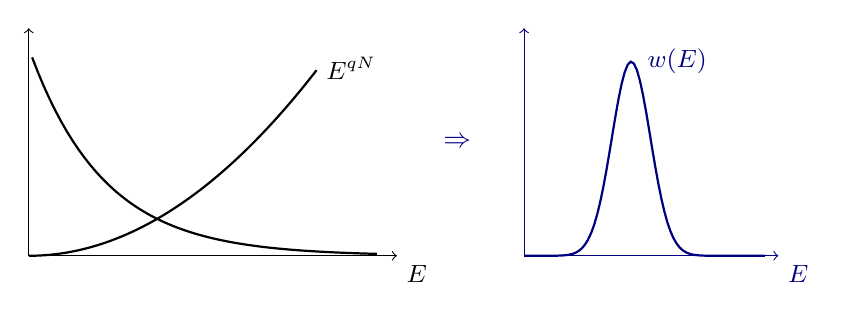
\begin{tikzpicture}[scale=0.85]
  \draw[->] (0,0) -- (5.5,0) node[below right] {\small $E$};
  \draw[->] (0,0) -- (0,3.4);
  \draw[thick,domain=0.05:5.2,samples=60] plot (\x,{3.1*exp(-0.9*\x)});
  \draw[thick,domain=0:4.3,samples=60] plot (\x,{0.15*\x*\x});
  \node[right] at (4.3,2.8) {\small $E^{qN}$};
  \node at (6.4,1.7) {\textcolor{NavyBlue}{$\Rightarrow$}};
  \begin{scope}[xshift=7.4cm,NavyBlue]
    \draw[->] (0,0) -- (3.8,0) node[below right] {\small $E$};
    \draw[->] (0,0) -- (0,3.4);
    \draw[thick,domain=0:3.6,samples=80] plot (\x,{2.9*exp(-6*(\x-1.6)*(\x-1.6))});
    \node[right] at (1.7,2.9) {\small $w(E)$};
  \end{scope}
\end{tikzpicture}
\end{center}

\begin{itemize}
  \item rovnovážný stav: $\max(w)$
  \item maximum: \quad $\displaystyle\pdv{E}\log w = \pdv{E}\Big(\overset{qN\log E}{\overset{\shortparallel}{\log\Sigma(E)}} - \beta E - \overset{\text{nez.\ na } E}{\log Z_c}\Big) = 0$
  \[
    \Rightarrow\quad \frac{qN}{E} = \beta \quad\Rightarrow\quad \vzorec{E_{eq} = \frac{qN}{\beta} = qk_BTN}
  \]
  \item $w$ je v dobrém přiblížení normální rozdělení \hfill \textcolor{NavyBlue}{$\swarrow$ viz centrální limitní věta $(+)$}
  \[
    \Rightarrow\quad -\frac{1}{\sigma^2} = \frac{\partial^2\log w}{\partial E^2}\Big|_{E = E_{eq}} = -\frac{qN}{E_{eq}^2}
    \quad\Rightarrow\quad \sigma = \frac{E_{eq}}{\sqrt{qN}}\sim\sqrt N
  \]
  \[
    \Rightarrow\quad \vzorec{\frac{\sigma}{E_{eq}}\propto N^{-1/2}\to 0} \ \text{ v td.\ limitě, \pozor{fluktuace v běžném experimentu neměřitelné}}
  \]
  \[
    \Rightarrow\quad w\sim\frac{1}{\sqrt{2\pi\sigma^2}}e^{-\frac{(E - E_{eq})^2}{2\sigma^2}}\Big|_{E = E_{eq}}\sim\frac{\sqrt N}{E_{eq}}\sim N^{-1/2}
  \]
  \[
    \Rightarrow\quad \max|\log w|\propto\tfrac12\log N\ll F\propto N
  \]
  \[
    \Big(N\sim N_A \Rightarrow \frac{\log N}{N}\sim 10^{-22}\Big)
  \]
\end{itemize}

\textcolor{NavyBlue}{$(+)$ \ $w(E)$ je hustota psti náh.\ proměnné $E = \sum_{i=1}^{N}\epsilon_i$, kde $\epsilon_i$ je energie $i$-té částice}

%----------------------------------------------------------------------
\strana{L10-12}
\begin{itemize}
  \item $\vzorec{F(T,V,N) = -k_BT\log Z_c}$ je fundamentální rovnice, lze tedy plně aplikovat formalismus TD pro systém v rovnováze s lázní
        \pozn{v originále chybí znaménko minus}

  \textbf{Př:} \quad $\bullet$ \ $F = U - TS$ \quad \& \quad $S = -\pdv{F}{T} = k_B\pdv{T}\big(T\log Z_c\big)$
  \[
    \Rightarrow\quad U = \langle E\rangle = F - T\pdv{F}{T}
  \]
  \pozn{v originále $F + T\,\partial F/\partial T$ -- překlep}
  \hspace*{2.4cm}$\uparrow$ pokud $H = H_0 + H_I$, potom je interpretace $U = \langle E\rangle = \langle H\rangle$ sporná, ale to ponecháme zatím stranou ($H_I$ \dots\ např.\ interakce s vnějším polem)
  \item střední hodnotu pozorovatelné $A = A(p,q)$ lze nicméně určit čistě SF metodami pomocí hustoty psti
  \[
    w_c(p,q) = \frac{1}{Z_c}e^{-\beta H(p,q)}
  \]
  \[
    \Rightarrow\quad \vzorec{\langle A\rangle = \int\dd\tau_N\,A(p,q)\,w_c(p,q)}
  \]
  \item spec.\ $A = H$ \ $\to$ \ $\langle E\rangle = \langle H\rangle = -\dfrac{\partial\log Z_c}{\partial\beta} = -\dfrac{1}{Z_c}\pdv{\beta}Z_c$
  \[
    = \frac{1}{Z_c}\int\dd\tau_N\,H(p,q)\,e^{-\beta H(p,q)} = \int\dd\tau_N\,w_c(p,q)\,H(p,q) \quad\checkmark
  \]
\end{itemize}

\underline{NB:} $\bullet$ dostáváme identitu \ ($\langle E\rangle\equiv U$) \quad $\vzorec{U = \pdv{\beta}(\beta F)}$
\begin{align*}
  U &= -\pdv{\beta}\log Z_c = \pdv{\beta}(\beta F) = F + \beta\pdv{F}{\beta} = F + \beta\pdv{F}{T}\pdv{T}{\beta} \\
  &= \Big/\ T = \frac{1}{k_B\beta} \Rightarrow \pdv{T}{\beta} = -\frac{1}{k_B\beta^2} = -k_BT^2
     \ \Rightarrow\ \textcolor{NavyBlue}{\boxed{\pdv{\beta} = -k_BT^2\pdv{T}}}\ \Big/ \\
  &= F - \frac{1}{k_BT}k_BT^2\pdv{F}{T} = F - T\pdv{F}{T} = F + TS
\end{align*}

%----------------------------------------------------------------------
\strana{L10-13}
$\Rightarrow$ oba postupy jsou ekvivalentní, kanonický soubor konzistentní s reprezentací $F(T,V,N)$ resp.\ $S[\frac1T]$

\begin{itemize}
  \item \textcolor{Red}{používat $\beta$ \underline{nebo} $T$, ale nemíchat; formalismus TD formulován s $T$, v SF přirozenější $\beta$!}
\end{itemize}

\subsubsection*{Fluktuace energie v kanon.\ souboru}
\[
  \langle(\Delta E)^2\rangle = \langle E^2\rangle - \langle E\rangle^2 \equiv
  \Big(\frac{1}{Z_c}\int\dd\tau_N\,H^2e^{-\beta H}\Big) - \Big(\frac{1}{Z_c}\int\dd\tau_N\,He^{-\beta H}\Big)^2
\]
\begin{itemize}
  \item $\displaystyle\pdv{\beta}\log Z_c = -\frac{1}{Z_c}\int\dd\tau_N\,He^{-\beta H}$ \hfill $\Big/\ \pdv{\beta}$
\end{itemize}
\[
  \frac{\partial^2}{\partial\beta^2}\log Z_c = \frac{1}{Z_c^2}\underset{\substack{\shortparallel\\ -\int\dd\tau_N He^{-\beta H}}}{\Big(\pdv{Z_c}{\beta}\Big)}\int\dd\tau_N\,He^{-\beta H}
  + \frac{1}{Z_c}\int\dd\tau_N\,H^2e^{-\beta H}
\]
\[
  \Rightarrow\quad \vzorec{\frac{\partial^2\log Z_c}{\partial\beta^2} = \langle E^2\rangle - \langle E\rangle^2 = \langle(\Delta E)^2\rangle}
\]
$\Rightarrow$ derivováním $Z_c$ dostáváme střední hodnotu i fluktuace
\begin{itemize}
  \item ale: \quad $\langle E\rangle = -\dfrac{\partial\log Z_c}{\partial\beta}$ \quad $\Rightarrow$ \quad $C_V = \pdv{T}\langle E\rangle = -k_B\beta^2\pdv{\langle E\rangle}{\beta}$
\end{itemize}
\[
  \Rightarrow\quad C_V = k_B\beta^2\frac{\partial^2\log Z_c}{\partial\beta^2}
  \quad\Rightarrow\quad \vzorec{\langle(\Delta E)^2\rangle = k_BT^2C_V}\ \textcolor{Red}{\textbf{!}}
\]
$\Rightarrow$ \kw{fluktuace energie souvisí s tepelnou kapacitou} za konst.\ objemu \quad (kanon.\ soubor $\leftrightarrow$ $V = \text{konst}$)

%----------------------------------------------------------------------
\strana{L10-14}
\begin{itemize}[nosep]
  \item[--] $T = \text{konst}$: čím větší $C_V$, tím více energie je třeba dodat, aby se zvýšila teplota \\
            ($\Rightarrow$ energie může více fluktuovat, aniž by se výrazně měnila teplota)
\end{itemize}

\underline{Pozn:} $\log Z_c$ je \kw{kumulant-generující funkcionál} pro $w(E)$: \quad
$\langle H^n\rangle_{w_c} = (-1)^n\dfrac{\partial^n}{\partial\beta^n}\log Z_c$

\noindent\rule{\linewidth}{0.4pt}

\underline{NB:}
\begin{itemize}
  \item lze zavést konzistentní formalismus, kdy $\Sigma(E,V,N)$ nazvu mikrokanonickou partiční sumou $Z_\mu(E,V,N)$ (v QM se skutečně jedná o součet přes stavy s danou energií $E$) \\
        $\Rightarrow$ fund.\ rovnice \quad $S(E,V,N) = k_B\log Z_\mu(E,V,N)$
  \item $Z_c(\beta,V,N) = \int\dd E\,Z_\mu(E,V,N)\,e^{-\beta E}$ \quad \dots\ Laplaceova trce \\
        $\to$ fund.\ rovnice \quad $S[\beta](\beta,V,N) = k_B\log Z_c(\beta,V,N)$ \\
        \hspace*{4.3cm}$\shortparallel$ \\
        \hspace*{3.3cm}$S(E,V,N) - \beta E$ \quad \dots\ Legendreova trce
  \item \uv{$-\beta E$} z Leg.\ trce FR se objevuje v exp.\ Laplaceovy trce partiční sumy
\end{itemize}

%----------------------------------------------------------------------
\strana{L10-15}
\subsection{Ekvivalence kanonického a mikrokanonického souboru}
\begin{itemize}
  \item pro $N\to\infty$, \ $\dfrac{(\Delta E)}{\langle E\rangle}\sim N^{-1/2}\to 0$
  \item přestože mají soubory různá pravděpodobnostní rozdělení, v TD limitě dávají oba soubory stejné hodnoty $\forall$ fyz.\ pozorovatelných, pokud je energie $E_*$ v mikrokanon.\ souboru taková, aby teplota
  \[
    \underbrace{\frac1T = \pdv{S_{mic}}{E}\Big|_{E = E_*}}_{\text{mikrokanon.\ soubor}} = \underbrace{\frac{1}{T_c} = k_B\beta_c}_{\text{kanon.\ soubor}}
  \]
  \item je dáno již diskutovanou zanedbatelnou šířkou $w_c(p,q)$: sice formálně integrujeme přes celý prostor, $w_c(p,q)$ je ale efektivně nulová pro $H(p,q)\neq E_{mic}$ \\
        $\Rightarrow$ ve finále počítáme opravdu totéž:
\end{itemize}
\begin{itemize}[label=$\to$]
  \item $Z = \int\dd E\,\Sigma(E)\,e^{-\beta E}$ \ $\Rightarrow$ def.\ $E_*$ skrze maximum $w_c(E)$
  \[
    \pdv{E}\big(\Sigma(E)\,e^{-\beta E}\big)\Big|_{E = E_*} = 0
    \ \overset{\text{metoda}}{\underset{\text{sedlového bodu}}{\Longrightarrow}}\
    Z\simeq\Sigma(E_*)\,e^{-\beta E_*}
  \]
  \item $\langle E\rangle = -\pdv{\beta}\log Z \simeq -\pdv{\beta}\big(\log\Sigma(E_*) - \beta E_*\big)$
  \[
    = -\pdv{\log\Sigma(E_*)}{E_*}\pdv{E_*}{\beta} + \beta\pdv{E_*}{\beta} + E_*
    = \Big/\ \overset{\text{mikro}}{\pdv{\log\Sigma(E_*)}{E_*} = \beta}\ \Big/ = E_*
  \]
\end{itemize}
\[
  \Rightarrow\quad \vzorec{\langle E\rangle_c = E_*}
  \qquad\text{opět vidíme soulad střední hodnoty a modu pravděp.\ rozdělení}
\]

%----------------------------------------------------------------------
\strana{L10-16}
\begin{align*}
  \to\quad S &= k_B\pdv{T}\big(T\log\overset{\textcolor{NavyBlue}{\swarrow Z_c\sim\Sigma(E_*)e^{-\beta E_*}}}{Z}\big)
     \simeq k_B\log\Sigma(E_*) - k_B\beta E_* + k_BT\pdv{T}\log\Sigma(E_*) \\
  &\quad - k_BT\pdv{T}(\beta E_*) = k_B\log\Sigma(E_*) - \cancel{k_B\beta E_*} - k_B\beta\pdv{\beta}\log\Sigma(E_*) \\
  &\quad + \cancel{k_B\beta E_*} + k_B\beta^2\pdv{E_*}{\beta}
     = k_B\log\Sigma(E_*) - k_B\beta\underset{\substack{\shortparallel\\ \frac{1}{k_BT} = \beta}}{\cancel{\pdv{\log\Sigma(E_*)}{E_*}}}\pdv{E_*}{\beta} \\
  &\quad + k_B\beta^2\cancel{\Big(\pdv{E_*}{\beta}\Big)}
\end{align*}
\[
  \Rightarrow\quad \vzorec{S_c = k_B\log\Sigma(E_*)}
\]

\subsection{Faktorizace partiční funkce}
\begin{minipage}{0.68\textwidth}
$H = \sum_{i=1}^{k}H_i$ \quad (např.\ neinteragující částice)
\end{minipage}
\begin{minipage}{0.3\textwidth}
\textcolor{NavyBlue}{$C_N$ je příslušný kombinatorický faktor!}
\end{minipage}
\[
  \Rightarrow\quad Z_c = \textcolor{NavyBlue}{C_N}\int\dd\tau_{N_1}\dots\dd\tau_{N_k}\,e^{-\beta\sum H_i}
  = \textcolor{NavyBlue}{C_N}\prod_{i=1}^{k}\int\dd\tau_{N_i}\,e^{-\beta H_i}
  = \vzorec{\textcolor{NavyBlue}{C_N}\prod_i(Z_c)_i}
\]
$\Rightarrow$ partiční funkce se faktorizuje na příspěvky nezávislých stupňů volnosti
\begin{enumerate}[label=\roman*)]
  \item velmi užitečné pro praktické výpočty
  \item $F(T,V,N_1,\dots,N_\ell) = \sum_iF_i(T,V,N_i)$ \\
        \hspace*{1.5cm}\underline{aditivita volné energie} id.\ plynu
\end{enumerate}
\begin{itemize}
  \item platí i pro $\Sigma$ v mikrokanonickém souboru \\
        $\Rightarrow$ aditivita entropie
\end{itemize}

\begin{priklad}[Id.\ plyn]
\color{NavyBlue}
\[
  Z_1 = \int\frac{\dd^3p\,\dd^3q}{h}\,e^{-\beta\frac{p^2}{2m}} = \frac{V}{h}\Big(\frac{2\pi m}{\beta}\Big)^{3/2} = \frac{V}{h}\big(2\pi mk_BT\big)^{3/2}
\]
\[
  \Rightarrow\quad Z_c = \frac{1}{N!}(Z_1)^N \quad\Rightarrow\quad
  F(T,V,N) = -k_BT\log Z_c = Nk_BT\big[f_0 - \log(T^{3/2}VN^{-1})\big] \quad\checkmark
\]
\pozn{v originále $h$ místo $h^3$ -- ponecháno}
\end{priklad}

%----------------------------------------------------------------------
\strana{L10-17}
\subsection{Gibbsova entropie}
\begin{itemize}
  \item $F = -\dfrac1\beta\log Z_c$ \qquad $Z_c = \int\dd\tau_N\,e^{-\beta H}$ \qquad $S = -\pdv{F}{T} = k_B\pdv{T}\big(T\log Z_c\big)$
  \item \begin{minipage}[t]{0.7\textwidth}
  \vspace{-4pt}
  $\displaystyle S = -\pdv{F}{T}$ \dots
  \begin{align*}
    S = -\pdv{F}{T} &= k_B\beta^2\pdv{F}{\beta} = -k_B\beta^2\pdv{\beta}\Big(\frac1\beta\log Z_c\Big) \\
    &= k_B\log Z_c - k_B\beta\pdv{\beta}\log Z_c \\
    &= k_B\log Z_c - \frac{k_B\beta}{Z_c}\pdv{\beta}\int\dd\tau_N\,e^{-\beta H}
  \end{align*}
  \end{minipage}
  \begin{minipage}[t]{0.25\textwidth}
  \color{gray}\small
  $S = \dfrac{U - F}{T}$ \\
  \hspace*{0.5cm}$\Uparrow$ \\
  $F = U - TS$
  \end{minipage}
\end{itemize}
\[
  \Rightarrow\quad S = \underset{\textcolor{gray}{= -F/T}}{k_B\log Z_c}
  + \underbrace{\frac{k_B\beta}{Z_c}\int\dd\tau_N\,He^{-\beta H}}_{\textcolor{gray}{\langle E\rangle/T\ \checkmark}} \qquad (+)
\]
\begin{itemize}
  \item $w_c(p,q) = \dfrac{1}{Z_c}e^{-\beta H}$ \ \& \ $\int\dd\tau_N\,w_c(p,q) = 1$
\end{itemize}
\begin{align*}
  \Rightarrow\quad S &= k_B\log Z_c + k_B\int\dd\tau_N\,w_c(p,q)\,\beta H \\
  &= k_B\int\dd\tau_N\,w_c(p,q)\big[\log Z_c + \beta H\big]
\end{align*}
\begin{itemize}
  \item $\log Z_c = -\log w_c(p,q) - \beta H$ \hfill $\swarrow$ \ $w_c = \dfrac{1}{Z_c}e^{-\beta H}$
\end{itemize}
\begin{veta}[Gibbsova entropie]
\[
  \Rightarrow\quad \vzorec{S = -k_B\int\dd\tau_N\,w(p,q)\log w(p,q)}
\]
\end{veta}
\underline{Pozn:} $\bullet$ funguje i pro mikrokanon.\ soubor: na přípustném fázovém podprostoru je hustota psti konstantní
\[
  w(p,q) = \frac{1}{\Sigma(E)} \quad\text{pro}\quad E = H(p,q)
\]
\[
  \Rightarrow\quad S = -k_B\log\frac{1}{\Sigma(E)}\int\dd\tau_N\,w(p,q) = k_B\log\Sigma(E)
\]

%----------------------------------------------------------------------
\strana{L10-18}
\subsection{\textcolor{OliveGreen}{Odbočka: kvantová statistická mechanika}}
{\color{OliveGreen}
\begin{itemize}
  \item v QM je čistý stav popsán vlnovou funkcí $\ket{\psi}$
  \item analog $w(p,q)$ je \kw{matice hustoty} (operátor hustoty)
  \[
    \vzorec{\hat\rho = \sum_kp_k\ket{\psi_k}\bra{\psi_k}} \qquad \sum_kp_k = 1
  \]
  \begin{itemize}
    \item $\ket{\psi_k}$ nemusí být vl.\ stavy $\hat H$, jsou to vl.\ stavy operátoru hustoty
    \item ve \underline{smíšeném stavu} popsaném $\hat\rho$ je čistý stav $\ket{\psi_k}$ zastoupen s pravděpodobností $p_k$
  \end{itemize}
  \item \underline{čistý stav} \quad $\hat\rho = \ket{\psi}\bra{\psi}$ \ $\Rightarrow$ \ $\langle F\rangle = \mel{\psi}{\hat F}{\psi}$
  \item \underline{smíšený stav} \quad $\langle F\rangle = \sum_kp_k\mel{\psi_k}{\hat F}{\psi_k} = \sum_k\mel{\psi_k}{\hat\rho\hat F}{\psi_k}$ \\
        \hspace*{6.6cm}$\uparrow$ $\braket{\psi_k}{\psi_\ell} = \delta_{k\ell}$
  \[
    \Rightarrow\quad \vzorec{\langle F\rangle = \operatorname{Tr}\big(\hat\rho\hat F\big)}
  \]
  \hspace*{3cm}NB: tento vztah nezávisí na bázi
  \item \underline{QM mikrokanonický soubor}
  \begin{itemize}
    \item[--] celková energie fixována $\Rightarrow$ dostupné jsou pouze čisté stavy $\ket{\psi_n}$ s energií $E_n = E$:
    \[
      \hat H\ket{\psi_n} = E_n\ket{\psi_n}
    \]
    \item[--] princip stejných pravděpodobností $\Rightarrow$
    \[
      p_n = \frac{1}{\Sigma(E)}; \quad \Sigma(E) = \sum_n\delta_{E,E_n}
      \quad\Rightarrow\quad \hat\rho = \frac{1}{\Sigma(E)}\sum_{E_n = E}\ket{\psi_n}\bra{\psi_n}
    \]
    \[
      \Rightarrow\quad \vzorec{[\hat\rho,\hat H] = 0}
    \]
  \end{itemize}
  \begin{itemize}[label=$\to$]
    \item $\Sigma(E)$ je počet stavů s energií $E$ $\Leftrightarrow$ stupeň degenerace hladiny $E$
    \item $S(E) = k_B\log\Sigma(E) = -k_B\sum_n\log p_n$ \pozn{tak v originále; správně $-k_B\sum_np_n\log p_n$}
    \item situace je zde v jistém smyslu jednodušší, definice $\Sigma(E)$ je jasnější (např.\ nerozlišitelnost je \uv{zakódována} v Hilb.\ prostoru)
  \end{itemize}
\end{itemize}
}

%----------------------------------------------------------------------
\strana{L10-19}
\subsection{\textcolor{OliveGreen}{Kanonický soubor v kvantové stat.\ mechanice}}
{\color{OliveGreen}
\begin{itemize}
  \item operátor hustoty: \quad $\vzorec{\hat\rho_c = \dfrac{1}{Z_c}e^{-\beta\hat H}}$
  \[
    Z_c = \operatorname{Tr}\big(e^{-\beta\hat H}\big) = \underset{\substack{\uparrow\\ \text{suma přes}\\ \text{stavy}}}{\sum_k}e^{-\beta E_k}
    = \sum_{E_n}\underset{\substack{\uparrow\\ \text{suma přes hladiny,}\\ \Sigma(E_n)\text{ je degenerace } E_n}}{\Sigma(E_n)}e^{-\beta E_n}
  \]
  \hfill ($\sim$ hustota stavů, je-li spektrum spojité)
  \item ostatní vztahy stejné:
  \[
    F = -k_BT\log Z_c \qquad \langle E\rangle = -\pdv{\beta}\log Z_c
  \]
  \item \uv{Gibbs}: \quad $\hat\rho = \dfrac{1}{Z_c}e^{-\beta\hat H}$ \ $\Rightarrow$ \ $p(E_n) = \dfrac{1}{Z_c}e^{-\beta E_n}$
\end{itemize}
\[
  \Rightarrow\quad \vzorec{S = -k_B\sum_np(E_n)\log p(E_n)}
  \qquad
  \fbox{\begin{minipage}{5.2cm}viz také Shannon/von Neumann \& entropie informace\end{minipage}}
\]
}
